\documentclass[../piano_di_qualifica.tex]{subfiles}
\begin{document}
\subsection{Test fase di analisi}
Qui di seguito verranno presentati i resoconti relativi ai test effettuati nella fase di analisi. \par

\begin{table}[!ht]
	\centering
	\begin{tabular}{|p{3cm}|p{3.3cm}|l|c|c|}
		\hline
		\rowcolor{lightgray}
		\textbf{Obiettivo}  & \textbf{Metrica} & \textbf{Risultato} & \textbf{Accettabile} & \textbf{Esito} \\
		\hline
		Ritardo maturato & MPR02 Varianza pianificazione  & 15 giorni  & \(\leq 4\) & Non Superato  \\
		\hline
		Budget intaccato   & MPR03 Varianza costi   &  Non è stato intaccato il budget totale    &  0\%  &  Superato\\
		\hline
		Rispetto obiettivi   & MPR07 Obiettivi soddisfatti     & 100\%   & 100\% & Superato  \\
		\hline
		QPR09 Rispetto delle norme  & MPR08 Norme rispettate   & 100\%  & 100\%   & Superato\\
		\hline
		Verifica documenti   & MPR10 Frequenza controllo    & Ogni Milestone e ogni modifica   & Ogni Milestone    & Superato \\
		\hline
		Leggibilità testo & MQP01 Indice di Gulpease  & 79,3  & \(\ge 60\)  & Superato \\
		\hline
		Correttezza ortografica   & MQP02 Errori ortografici   &     0    &  0 & Superato  \\
		\hline
	\end{tabular}
	\caption{Metriche qualità di processo}
\end{table}


\subsection{Esiti verifica indici di Gulpease}
\label{sub:verif_gul}

\begin{center}
	\begin{longtable}{|l|c|c|}
		\hline
		\rowcolor{lightgray}
            \textbf{Documento} & \textbf{Risultato} &  \textbf{Esito} \\
            \hline 
            Analisi Dei Requisiti v1.0.0 & 86   & Superato \\
            \hline
            \hline 
            Piano di Progetto v1.0.0 & 70 & Superato \\
            \hline 
            Piano di Qualifica v1.0.0 & 69 & Superato \\
            \hline 
            Norme di Progetto v1.0.0 & 71 & Superato \\
            \hline 
            Studio di Fattibilità v1.0.0 & 71 & Superato \\
            \hline 
            Glossario v1.0.0 & 66 & Superato \\
            \hline 
            Verbale Interno 2020-11-25 v1.0.0 & 73 & Superato \\
            \hline 
            Verbale Interno 2020-12-10 v1.0.0 & 86 & Superato \\
            \hline 
            Verbale Interno 2020-12-21 v1.0.0 & 72 & Superato \\
            \hline 
            Verbale esterno 2020-12-17  v1.0.0 & 76 & Superato \\
            \hline
	    Verbale esterno 2021-01-08  v1.0.0 & 60 & Superato \\
            \hline
            \hline

\caption{Tabella contenente le valutazioni dei documenti}
\end{longtable}
\end{center}

\begin{figure}[H]
\centering
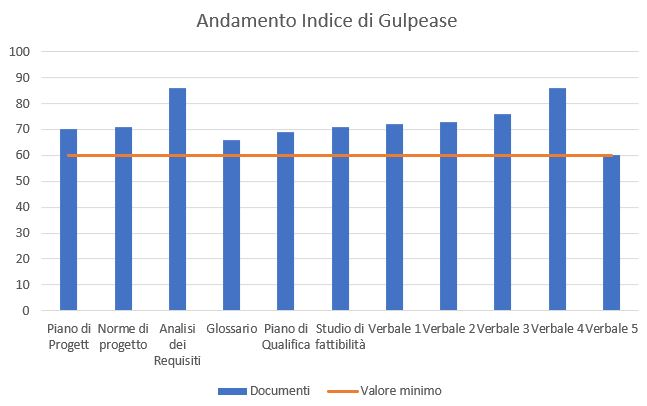
\includegraphics[width=12cm]{componenti/media_gul}
\caption{ Andamento Indice di Gulpease}
\end{figure}



\end{document}